\documentclass{beamer}
\usepackage{graphicx}
\usepackage{amsmath}

\title{Recognizing Affect in Spoken Language}
\author{Benjamin Goldenberg}
\institute{Center for Spoken Language Understanding}
\date{13 August 2009}

\begin{document}
\begin{frame}
	\titlepage
\end{frame}

\begin{frame}{Overview}
	\begin{itemize}
		\item Accurately recognizing affect is important for many applications, ranging from text-to-speech to monitoring mental health.
		\item This project studies how older people vary in their expressions of affect by exposing them to stimuli meant to ellicit positive or negative emotion.
		\item We have built a pipeline to train Support Vector Machines on a variety of lexical and semantic textual features.
		\item We have tested this pipeline on data made available by Cecilia Alm and preliminary data from the Social Engagement meter.
	\end{itemize}
\end{frame}

\begin{frame}{Positive slide}
	\begin{figure}[htbp]
		\centering
			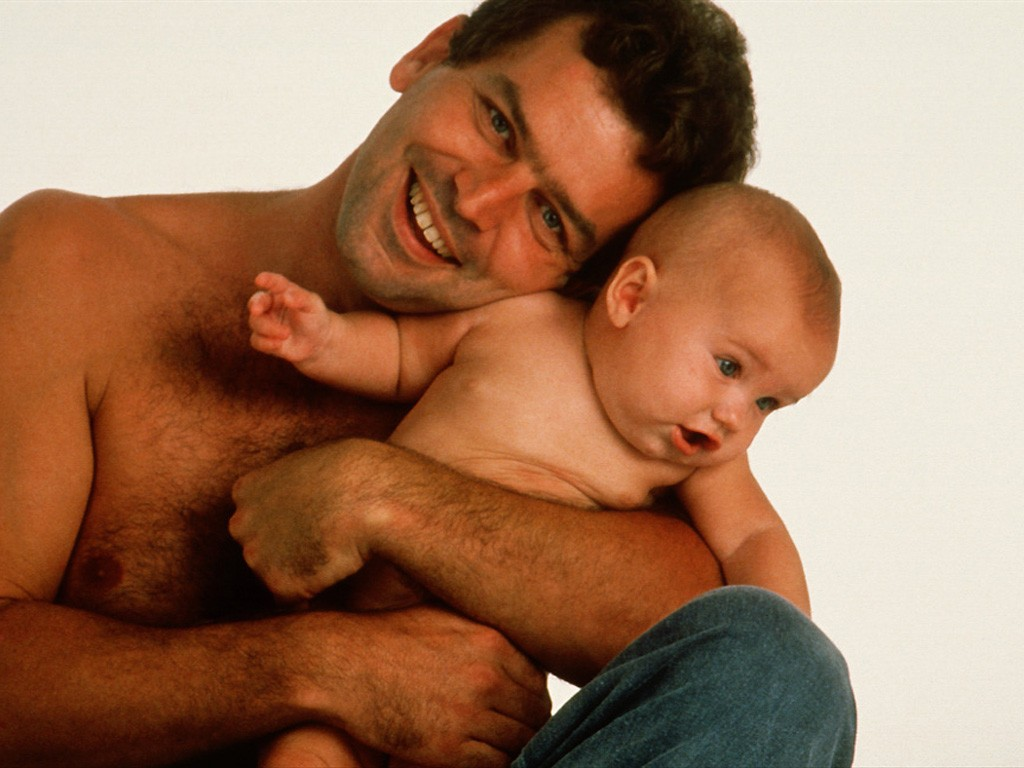
\includegraphics[height=3in]{figures/positive.jpg}
		\label{fig:figures_positive}
	\end{figure}	
\end{frame}

\begin{frame}{Negative slide}
	\begin{figure}[htbp]
		\centering
			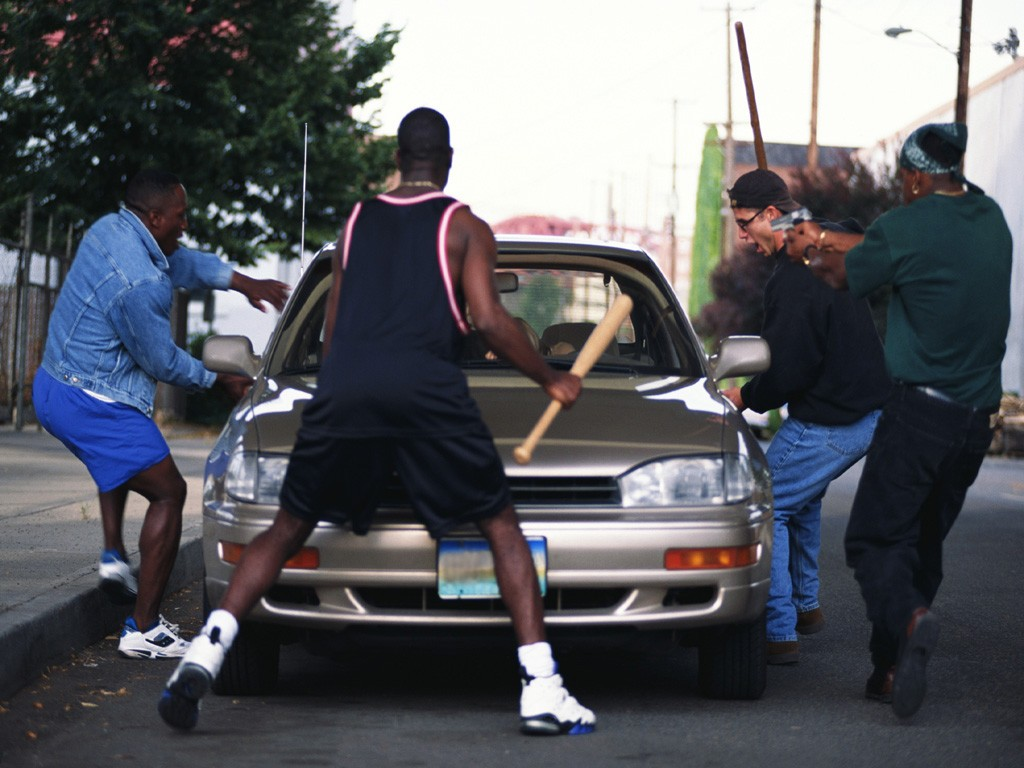
\includegraphics[height=3in]{figures/negative.jpg}
		\label{fig:figures_negative}
	\end{figure}
\end{frame}

\begin{frame}{Rating stage}
	\begin{figure}[htbp]
		\centering
			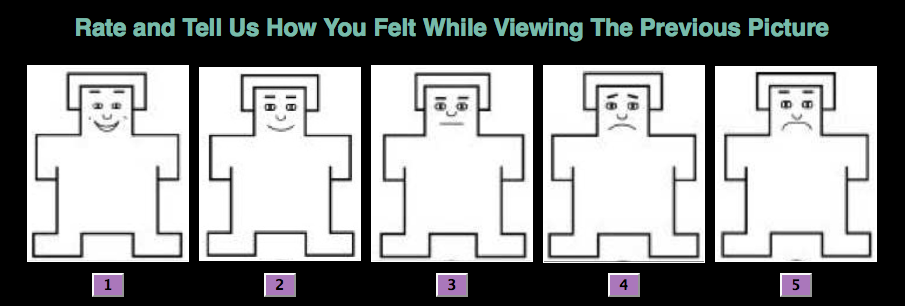
\includegraphics[height=1.35in]{figures/rating.png}
		\label{fig:figures_rating}
	\end{figure}	
\end{frame}

\begin{frame}{Support Vector Machines}
	\begin{figure}[htbp]
		\centering
			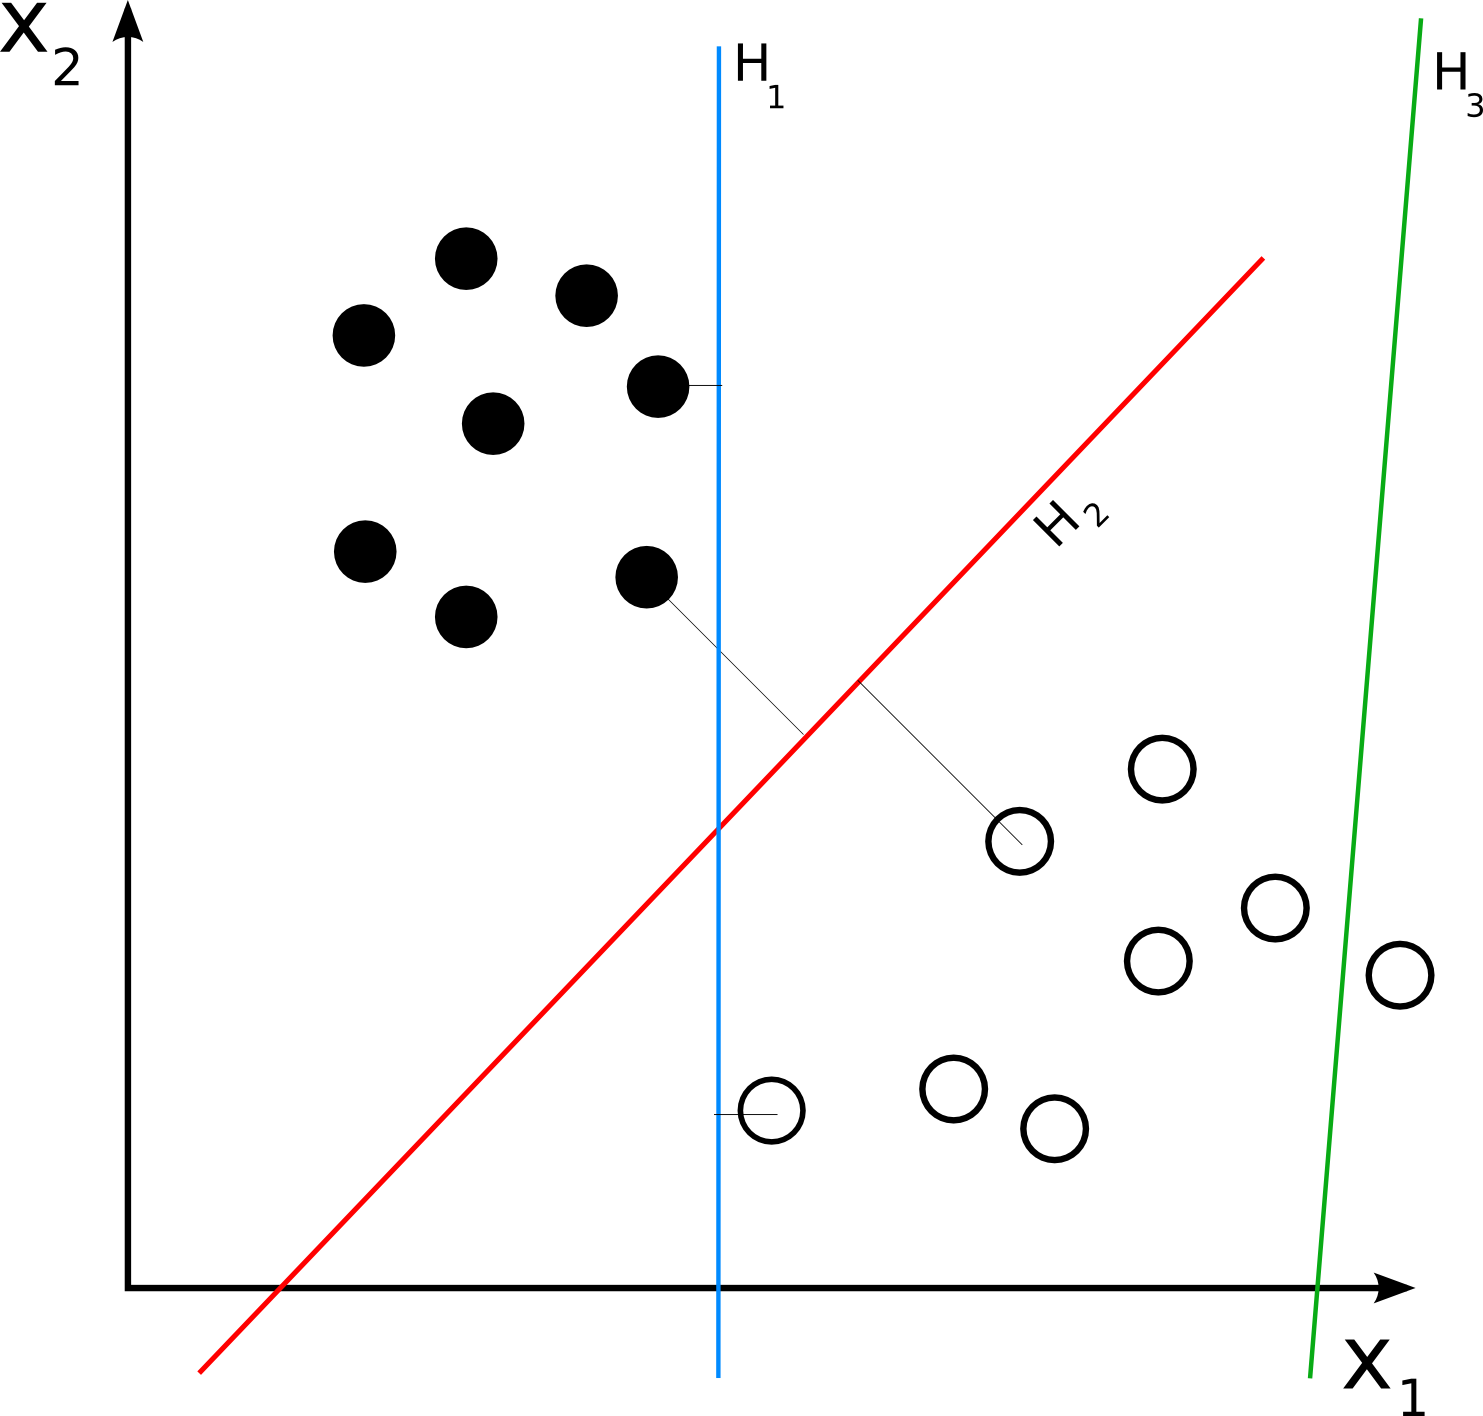
\includegraphics[height=3in]{figures/svm.png}
		\label{fig:figures_svm}
	\end{figure}
\end{frame}

\begin{frame}{Finite State Transducers}
	\begin{figure}[htbp]
		\centering
			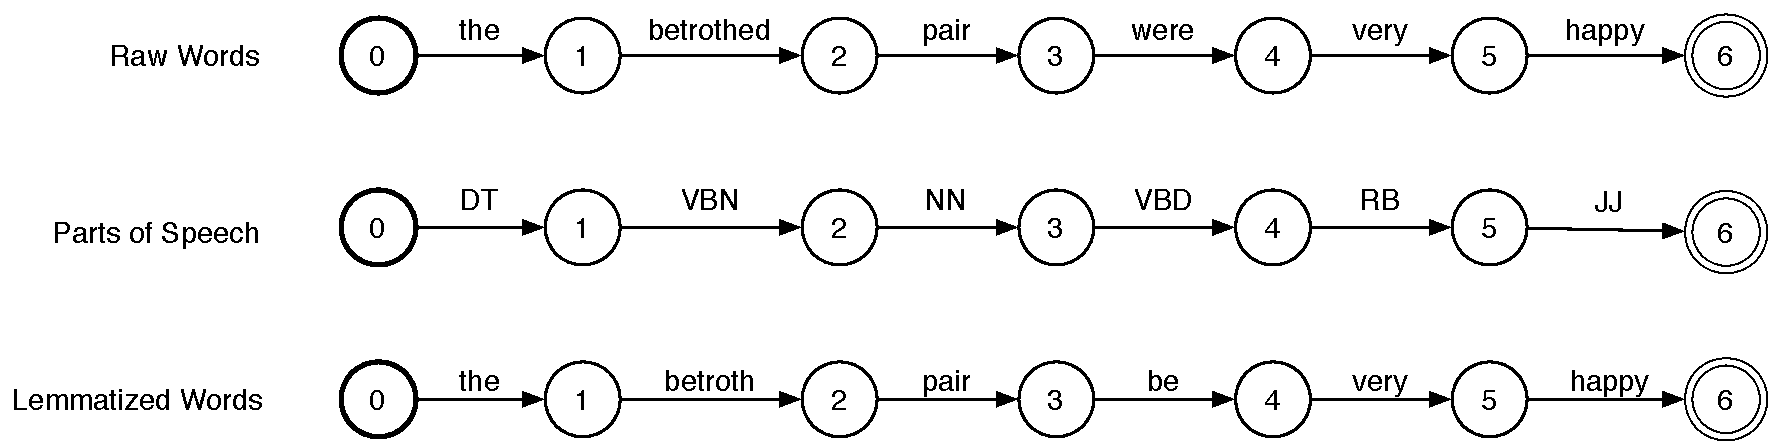
\includegraphics[width=4in]{figures/words-pos-lemmas.pdf}
		\label{fig:figures_words-pos-lemmas}
	\end{figure}
\end{frame}

\begin{frame}{More complicated transducers}
	\begin{figure}[htbp]
		\centering
			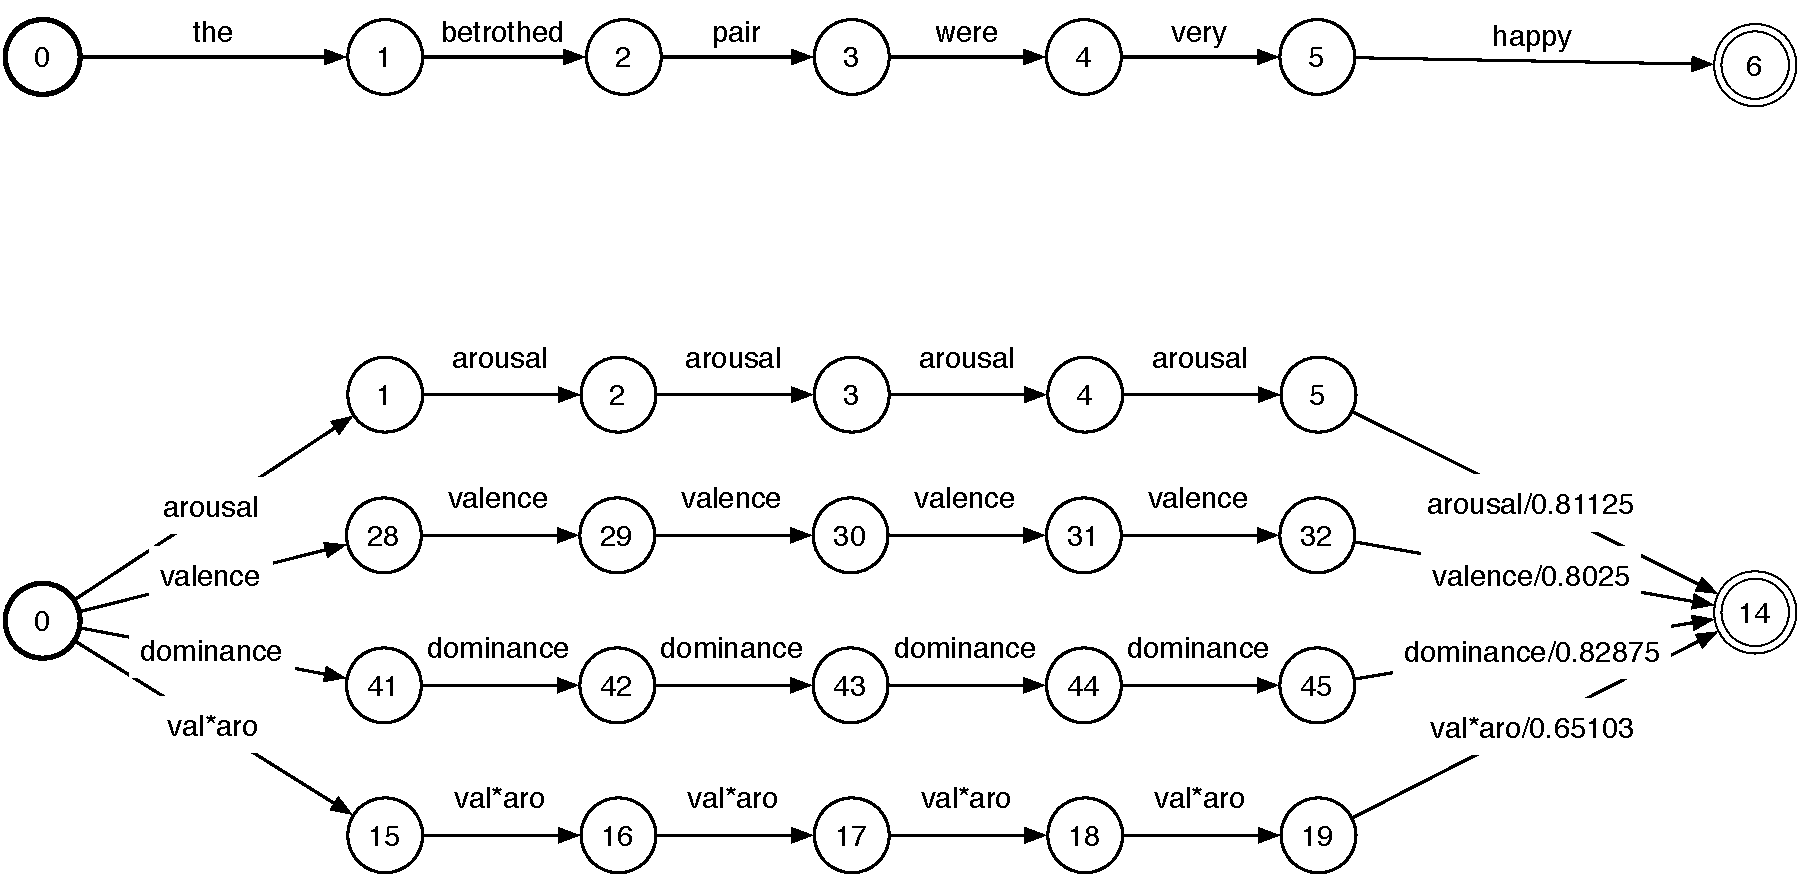
\includegraphics[width=4in]{figures/words-anew.pdf}
		\caption{Multipath FST labelling using the ANEW dataset}
		\label{fig:figures_words-anew}
	\end{figure}
	
\end{frame}
\begin{frame}{Alm data (2002)}
	\begin{figure}[htbp]
		\centering
			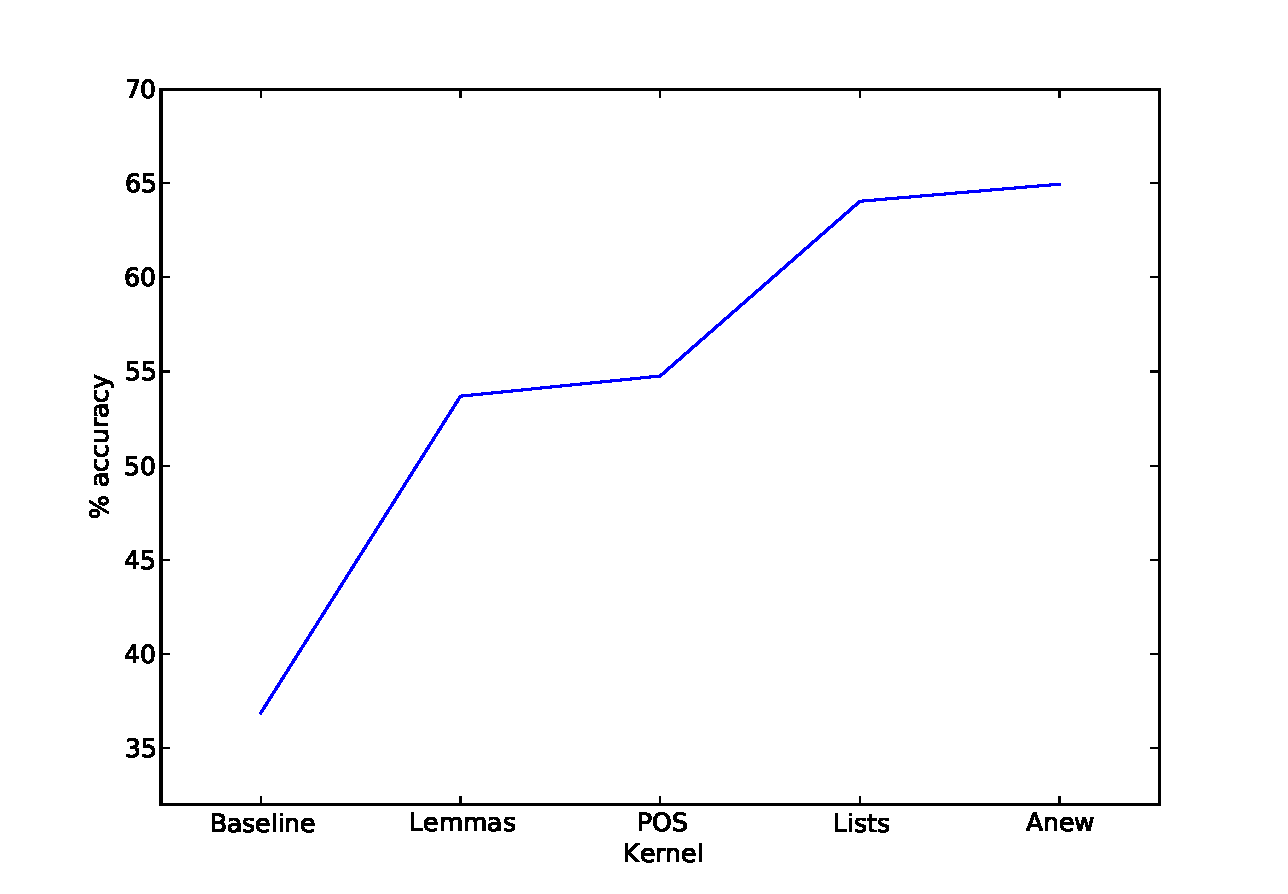
\includegraphics[width=4in]{figures/alm-kernels.pdf}
		\caption{Consecutive summing of kernels.}
		\label{fig:figures_words-anew}
	\end{figure}
\end{frame}

\begin{frame}{Social Engagement Meter data (2009)}
	\begin{figure}[htbp]
		\centering
			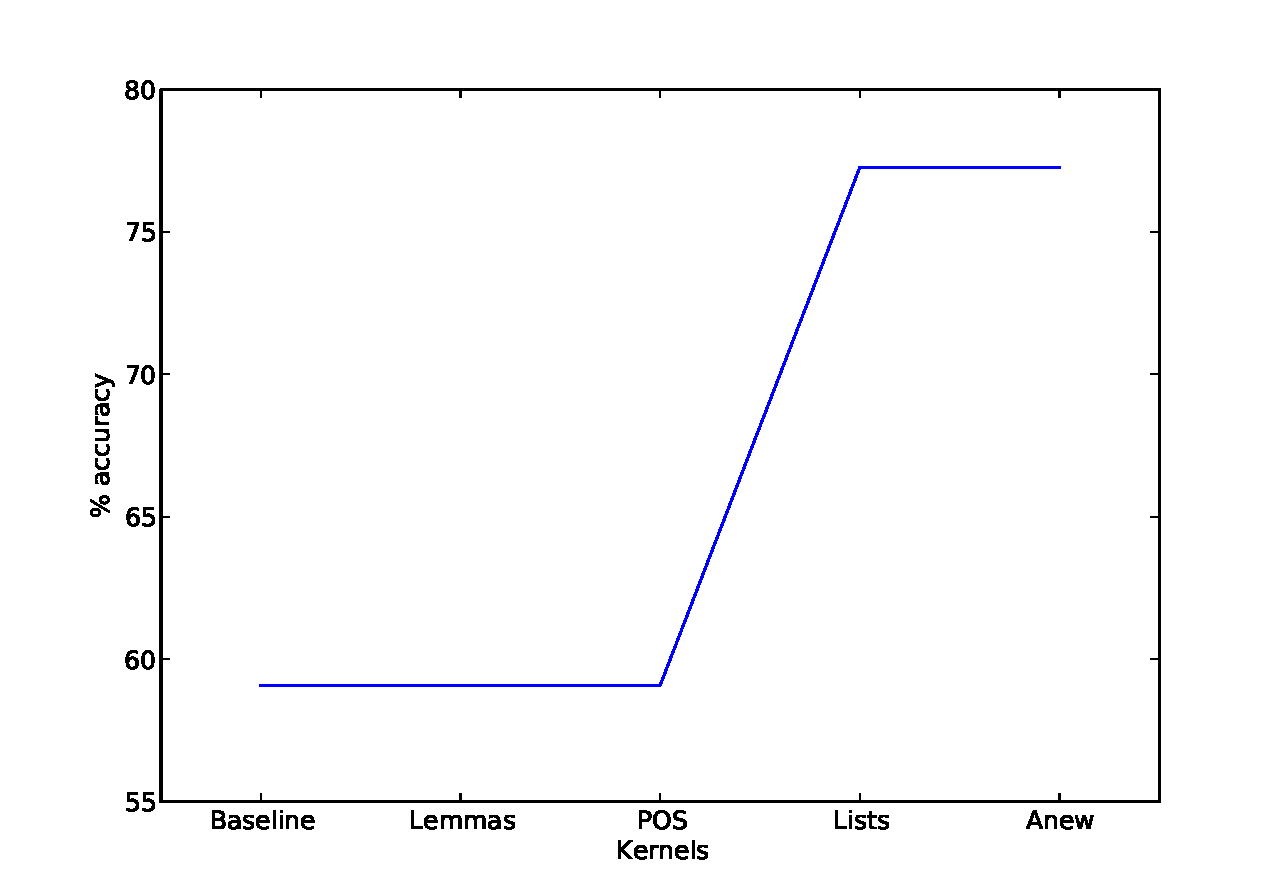
\includegraphics[width=4in]{figures/subject-kernels.pdf}
		\caption{Consecutive summing of kernels.}
		\label{fig:figures_words-anew}
	\end{figure}
\end{frame}

\begin{frame}{Future Work}
	\begin{itemize}
		\item Explore more combinations of kernels.
		\item Use probabilistic word lattices from the speech recognizer.
		\item Combine acoustic and lexical classification.
	\end{itemize}
\end{frame}

\begin{frame}{References}
	\begin{itemize}
		\item Alm, C. (2002). \emph{Affect in Text and Speech}. PhD thesis, University of Illinois at Urbana-Champaign, Urbana, Illinois.
		\item Cortes, C., Haffner, P., and Mohri, M. (2004). Rational kernels: Theory and algorithms. \emph{Journal of Machine Learning Research}, 1:1–50.

		\item Shafran, I., Riley, M., Mohri, M. (2003) Voice Signatures. \emph{Proc. of IEEE Automatic Speech Recognition and Understanding Workshop}, 31-36 
	\end{itemize}
\end{frame}

\begin{frame}
	\begin{center}
		\Large{Questions?}
	\end{center}
\end{frame}
\end{document}